%! TEX root = 0-main.tex
\chapter{Heat Engines and Refrigerators}

A heat engine is a thermodynamic cycle that converts heat into useable work. Quasi-static processes are useful to study these cycles. 

A quasi-static proces is a process that happens slowly enough where the system always remains in equilibium; the entropy does not increase, and so the process is \emph{reversible}. While such a process does not truly exist, it is a useful construction. All real thermodynamic processes result in the increase of entropy, and thus are irreversible.

\section{Heat Capacity}
The heat capacity of an object is defined as
\begin{equation}
	C=\frac{\dbar{Q}}{\d{T}}
\end{equation}
Often, we are interested in constant volume and constant pressure processes. Respectively, \(C_V\) and \(C_P\) denote heat capacity at constant volume and constant pressure.

Additionally, we can make the heat capacity into the intensive property \emph{specific heat capacity} \(c\), which is the heat capacity per unit mass. 

Under the assumption that particles are not exchanged, under constant volume \(\d{V}=0\), we get the heat capacity to be
\begin{equation}
	C_V=\frac{\dbar{Q}}{\d{T}}=\der{U}{T}
\end{equation}

Using the energy for an ideal monatomic gas,\footnote{The reason that we specify a monatomic gas is due to the equipartition theorem. Each quadratic degree of freedom has \(\frac{1}{2}k_BT\) worth of energy; an ideal diatomic gas would have energy \(U=\frac{5}{2}k_BT\), as there are 5 quadratic degrees of freedom (3 translation and 2 rotation)}
\[U=\frac{3}{2}Nk_BT\]
we have
\begin{equation}
	C_V=\frac{3}{2}k_B N
\end{equation}

For constant pressure, we can use the ideal gas law
\[PV=Nk_BT\]
to write
\begin{equation}
	C_P=\frac{\d U +P\d{V}}{\d{T}} = \frac{\d{U}+Nk_B\d{T}}{\d{T}}=C_V+Nk_B
\end{equation}
This can be rearranged to give Mayer's relation for an ideal gas:
\begin{equation}
	nR=C_P-C_V
\end{equation}
Thus, we must have
\begin{equation}
	C_P>C_V
\end{equation}

Further, we can compute
\begin{equation}
	\gamma\equiv\frac{C_P}{C_V}=\frac{C_V+Nk_B}{C_V}=\frac{5}{3}=\frac{f+2}{f}
\end{equation}
This quantity, known as the \emph{adiabatic index},  plays an important role in adiabatic processes.

\section{Adiabatic Processes}
In an adiabatic process, no heat is transfered. In an adiabatic expansion or compression, the volume of the gas is changed very rapidly, as to not allow any time for heat to transfer.

Differentiating the ideal gas law, we then have:
\[P\d{V}+V\d{P}=nR\d{T}=(C_P-C_V)\d{T}\]
Because there is no heat, we can write
\[C_V=\der{U}{T}=-\frac{P\d{V}}{\d{T}}\]
Plugging this in, we get:
\[P\d{V}+V\d{P}=(\gamma-1)C_V\d{T}=(1-\gamma)P\d{V}\]
moving terms and simplifying,
\[\gamma\frac{\d{V}}{V}+\frac{\d{P}}{P}=0\]
Integrating, we get
\begin{equation}
	P_1V_1^\gamma=P_2V_2^\gamma\label{eq10:adiabaticexp}
\end{equation}
Plugging in the ideal gas law, we can write the effect on temperature as:
\begin{equation}
	T_1V_1^{\gamma-1}=T_2V_2^{\gamma-1}
\end{equation}
Thus, as volume decreases, the temperature increases. This is because work is being done on the gas to compress it. In contrast, with adiabatic expansion, the gas does work and the temperature must decrease.

Adiabatic expansion can be contrasted with \emph{free expansion}, where a gas is allowed to expand into a vacuum. Because there is no pressure, the work a gas does is zero, and the temperature does not change.

\section{Thermodynamic Cycles}
Thermodynamic cycles operate on two principles. 
Because a thermodynamic cycle is cyclic, the entropy change after a complete cycle (assuming quazi-static/ideal processes) must be zero (although it can be non-zero during the cycle).
\begin{equation}
	\d{S}=\frac{\dbar Q_H}{T_H}+\frac{\dbar Q_L}{T_L}=0
\end{equation}
Further, the work is the amount of energy extracted from the heat:
\begin{equation}
	\dbar{W}=\dbar{Q_H}+\dbar{Q}_L
\end{equation}

\subsection{Heat Engine}
A heat engine is a thermodynamic cycle that converts (useable) heat into work. The prototypical heat engine is the Carnot Cycle. From the hot reservoir, we have \(\dbar Q_H>0\) coming into the engine, and \(-\dbar Q_L>0\) removed from the system. 

The ideal efficiency of a heat engine is the Carnot efficiency, and is defined as the ratio of the work extracted from the total amount of heat entering the engine:
\begin{equation}
	\eta \equiv \frac{\dbar{W}}{\dbar{Q_H}}=1-\frac{T_L}{T_H}
\end{equation}

The first law tells us that \(\dbar{W}\leq \dbar{Q}_{H}\) (you can't win), and the second law says that \(\d{S}>0\) (you can't break even).

\subsection{Refrigerator}
By reversing a heat engine, we can use mechanical work to pump heat from a cold reservoir to a hot reservoir. The coefficient of performance for a refrigerator is defined to be the amount of heat extracted from the cold reservoir divided by the amount of work required to do so:
\begin{equation}
	\epsilon_R=\frac{\dbar{Q}_L}{-\dbar{W}}=\frac{T_L}{T_H-T_L}
\end{equation}
In a refrigerator, a compressor copresses a refrigerant vapour, increasing the temperature above ambient. The ambient air cools the compressed vapour until it condenses in the condenser. Then, the liquid cools as it passes through an expansion valve and enters the refrigerator. The liquid refrigerant absorbs heat from the refrigerator to evaporate, and the gaseous refrigerant re-enters the compressor.

\subsection{Heat Pump}
A heat pump operates in a similar way, except it uses the heat outside a system to heat a system. Its coefficient of performance is defined to the amount of heat pumped into the hot reservoir divided by the amount of work required to do so:\footnote{Note that while the difference between a refrigerator and heat pump may seem superficial at first, the difference between the two cycles is the reservoir that we care about.}
\begin{equation}
	\epsilon_{HP}=\frac{-\dbar{Q}_H}{\dbar{W}} = \frac{T_H}{T_H-T_L}
\end{equation}
Interestingly, a heat pump often has a much higher efficiency than an electrical resistive heating element.

\section{Carnot Cycle}
The Carnot Cycle is a four-stage process:
\begin{enumerate}
	\item Isothermal expansion in contact with a hot reservoir
	\item Adiabatic expansion
	\item Isothermal compression in contact with cold reservoir
	\item Adiabatic compression
\end{enumerate}


\subsubsection{Isothermal Expansion}
Because the change in temperature is zero, the change in \(U=\frac{3}{2}nRT\) is also zero, thus,
\[W_{12}=\int_{V_A}^{V_B}P\d{V}=Nk_BT\int_{V_A}^{V_B}\d{V} V^{-1} = Nk_BT\ln\left(\frac{V_B}{V_A}\right)=Q_H\]

Further, the change in entropy is given:
\[\Delta S_{12}=\frac{Q_H}{T_H}\]

\subsubsection{Adiabatic Expansion}
The ideal gas is thermally isolated and allowed to expand adiabatically. Thus, the temperature decreases to \(T_L\). Using the equation for adiabatic expansion (and plugging in \(\gamma=5/3\))
\[T_HV_2^{2/3}=T_LV_3^{2/3}\then V_3=V_2\left(\frac{T_H}{T_L}\right)^{3/2}\]

The work being done is more complicated to calculate and has been temporarily omitted

Because no heat is transfered, the change in entropy is
\[\Delta S_{23}=0\]

\subsubsection{Isothermal Compression}
Once again, temperature is held constant while the gas is expanded. Similar to the isothermal expansion, we can find the work done as
\[W_{34}=Nk_BT_L\ln\left(\frac{V_4}{V_3}\right)=-Q_L\]

and the entropy is
\[\Delta S_{34} = -\frac{Q_L}{T_L}\]

\subsubsection{Adiabatic Compression}
Again, the volume and temperature obey the relation
\[T_LV_4^{2/3}=T_HV_1^{2/3}\]
and the change in entropy is
\[S_{41}=0\]

\subsection{Total Cycle}
Over a complete cycle, the work done by the gas is given
\begin{equation}
	W=W_{12}+W_{23}-W_{34}-W_{41}
\end{equation}
and the change in internal energy tells us
\[0 = \Delta U=\Delta Q-W\then W=Q_H-Q_L\]
The total change in entropy is also zero:
\[0=\Delta S = S_{12}+S_{23}+S_{34}+S_{41}=\frac{Q_H}{T_H}-\frac{Q_L}{T_L}\]
Thus, we have
\begin{equation}
	\frac{Q_H}{Q_L}=\frac{T_H}{T_L}
\end{equation}
and the volumes are related by
\[\frac{T_H}{T_L}=\frac{Q_H}{Q_L}=\frac{Nk_BT_H\ln\left(\frac{V_2}{V_q}\right)}{Nk_BT_L\ln\left(\frac{V_3}{V_4}\right)}\]
\begin{equation}
	\frac{V_2}{V_1}=\frac{V_3}{V_4}
\end{equation}

This cycle can be visualized in the PV diagram in Figure~\ref{fig10:carnotpv} and the TS diagram in Figure~\ref{fig10:carnotts}

\begin{figure}[!htbp]
	\begin{center}
		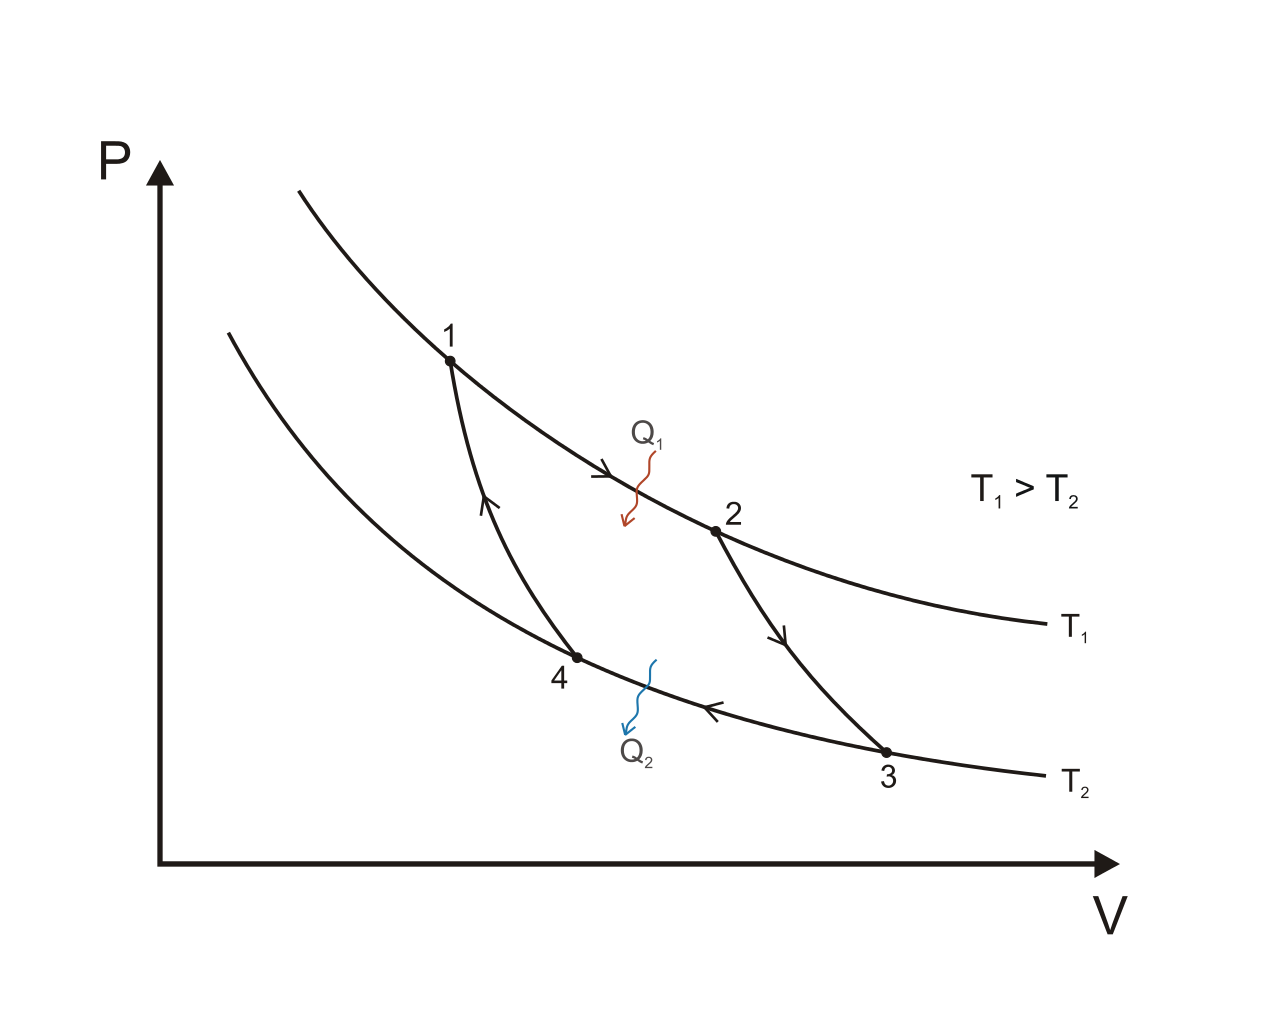
\includegraphics[scale=0.3]{diagrams/CarnotPV.png}
	\end{center}
	\caption{PV diagram of Carnot Cycle}\label{fig10:carnotpv}
\end{figure}
\begin{figure}[!htbp]
	\begin{center}
		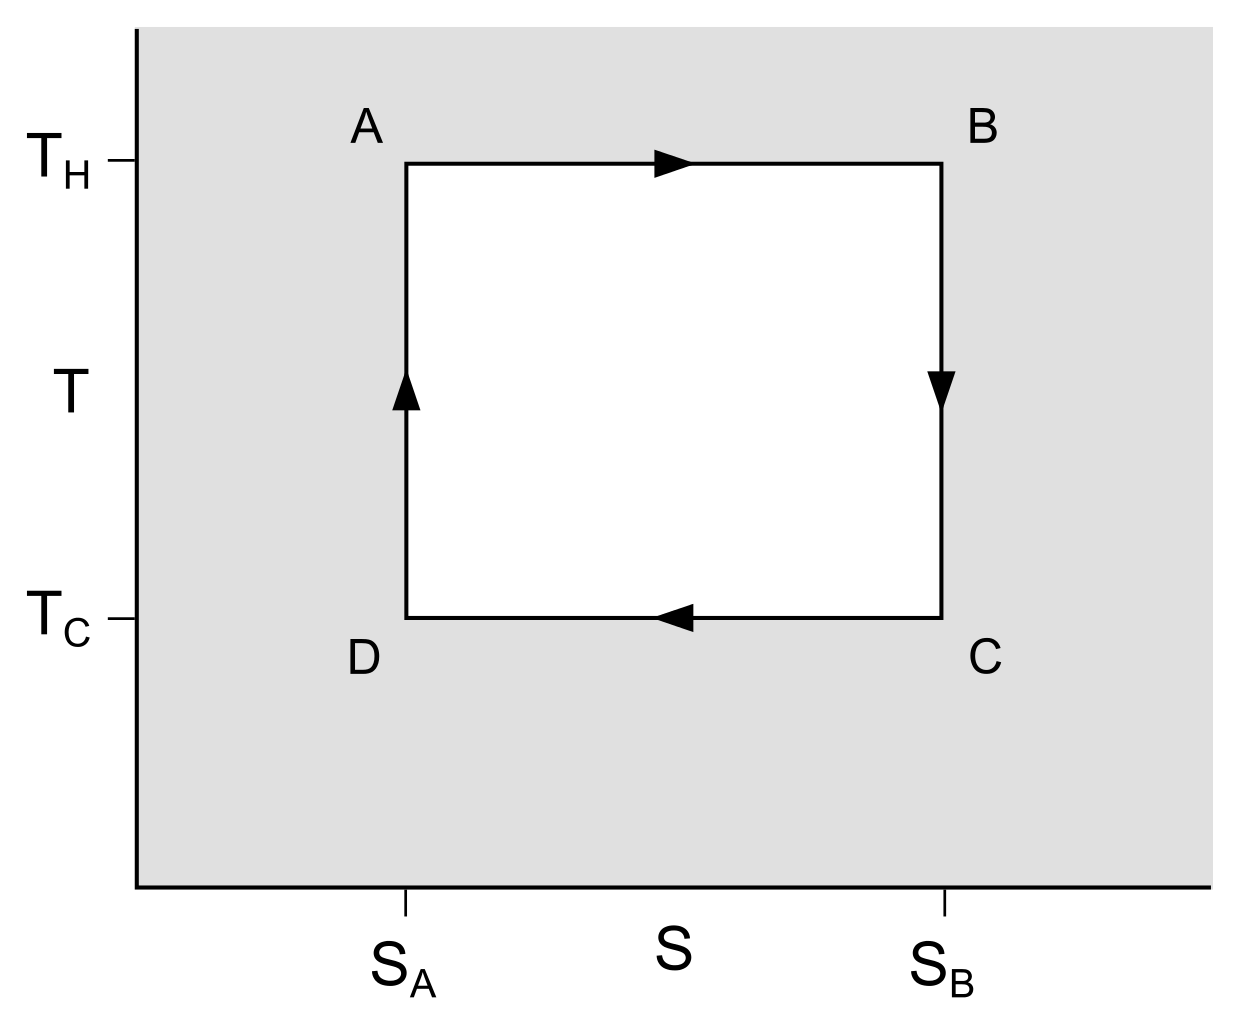
\includegraphics[scale=0.3]{diagrams/CarnotTS.png}
	\end{center}
	\caption{TS diagram of Carnot Cycle}\label{fig10:carnotts}
\end{figure}

\begin{aside}[Negative Temperature]
	Recall that temperature is defined by
	\[k_B\beta = \frac{1}{T}=\pder{S}{E}\]
	If entropy decreases with an increase in energy, then the temperature is \emph{negative}. If a system with negative temperature is put in thermal contact with a system with positive temperature, the equilibrium point is not zero, but rather infinite! Rather than colder than absolute zero, \emph{a negative temperature is hotter than infinite kelvin}.

	The discontinuity of traditional temperature motivates the importance of thermodynamic beta, as absolute zero is \(+\infty\), the value at \(0\) is continuous. 
\end{aside}

